\documentclass{kththesis}

\usepackage{blindtext} % This is just to get some nonsense text in this template, can be safely removed
\usepackage{graphicx}
\usepackage{tabularx}
\usepackage{multirow}
\usepackage{csquotes} % Recommended by biblatex
\usepackage{biblatex}
\usepackage{listings}
\usepackage{algorithmicx}
\usepackage{algorithm}
\usepackage{algpseudocode}
\usepackage[counterclockwise, figuresleft]{rotating}
\addbibresource{USBMon.bib} % The file containing our references, in BibTeX format


\title{Characterization and mitigation of timing delays in Software Defined Radio architecture}
% \alttitle{Detta är den svenska översättningen av titeln}
\author{Saptarshi Hazra}
\email{hazra@kth.se}
\supervisor{Peng Wang, Simon Duquennoy, Niklas Wirström}
\examiner{Marina Petrova}
\programme{EIT Digital Master in Embedded System}
\school{School of Electrical Engineering and Computer Science}
\date{\today}


\begin{document}

% Frontmatter includes the titlepage, abstracts and table-of-contents
\frontmatter

\titlepage

% \begin{abstract}
%   English abstract goes here.

%   \blindtext
% \end{abstract}

% \begin{abstract}
%     Träutensilierna i ett tryckeri äro ingalunda en oviktig faktor,
%     för trevnadens, ordningens och ekonomiens upprätthållande, och
%     dock är det icke sällan som sorgliga erfarenheter göras på grund
%     af det oförstånd med hvilket kaster, formbräden och regaler
%     tillverkas och försäljas Kaster som äro dåligt hopkomna och af
%     otillräckligt.
%   \end{abstract}


\tableofcontents


% Mainmatter is where the actual contents of the thesis goes
\mainmatter


\chapter{Introduction}

Software Defined Radio (SDR) provides flexibility in terms of design and allows for carefully analyzing RF signals and experimenting with decoding and modulation techniques. For the military sector, where communication systems need to have a longer service life time than in the commercial sector, SDR helps to protect investments by prolonging the useful service life of communication systems. This is facilitated through SDR allowing the possibility to change protocols on already acquired SDR equipment. It also allows for flexibility of porting an already existing SDR protocol to another more capable SDR platform without much hassle. A major motivation within the commercial communications arena, is the rapid evolvement of communications standards, making SW upgrades of base stations a more attractive solution than the costly replacement of base stations\cite{ulversoy_software_2010}. SDR also opens up the possibility of Cognitive Radios, a context sensitive radio system that can adapt depending on the radio channel conditions and applications. 
A fundamental challenge of SDR systems is computational horsepower, because it needs to process complex data waveforms at a fixed cost of both time and power, which is difficult as generally specialized hardware is much more efficient in terms of performance and power consumption. \\
This project tries to the enabler for technology agnostic radio head which would allow to develop future proof the communication systems and also since the raw sample data is available to the host, that can be analyzed to open up new application domain in radio channel evaluation and cognitive radios. \\
Software Defined Radio based communication systems are limited by the round trip delay which consists of communication delay between the SDR platform and the host computer and also processing delay in the host computer. These delays don’t usually comply with the standard MAC definitions hence complete standard complaint performance is not possible. Understanding and mitigation of these
delays is missing for recent SDR platforms like LimeSDR.

\section{Research Question}
\begin{itemize}
\item{Where the the communication bottlenecks in SDR based communication systems?}
\item{ How can we mitigate these timing delays?}
\end{itemize} 
\chapter{Background}
This chapter presents the relevant background information that are useful in the understanding of the report. First, it introduces USBMon kernel utility and how it provides event updates. Second, it explains the LimeSDR software defined radio platform and specifically its USB communication architecture.

\section{USBMon}
It is kernel facility provided to collect I/O traces on the USB Bus\cite{_usbmon}. USBMon reports the requests made to and by the USB Host Controller Drivers(HCD). It provides two kinds of API's : binary and character. The binary API is accessed by character devices located in the /dev namespace. The character API provides human readability and uniform format for the traces.The kernel data from the USBMon text data is made available to the userspace using debugfs\cite{_debugfs} utility.

\begin{figure}[h!]
\centering
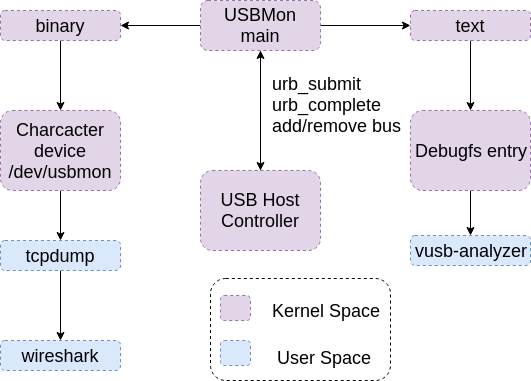
\includegraphics[width=\textwidth]{USBMon.png}
\caption{USBMon Architecture(Adapted from \cite{basak_usb_2018}).}
\end{figure}

\subsection{Text Data Format}
\begin{table}
\centering
\begin{tabular}{|c|c|c|c|c|}
\hline
URB Tag & Timestamp & Event Type & Address & URB Status\\
\hline
ffff8fbdbbae4000 & 2942307806 & S & Bo:3:008:15 & -115\\ 
\hline
\end{tabular}
\begin{tabular}{|c|c|c|}
\hline
Data Length & Data Tag & Data\\
\hline
64 & = & 21000100 00000000 002a0484 00000000 000000\\
\hline
\end{tabular}
\caption{Text USB Trace Example.}
\end{table}

\begin{itemize}
\item {\textit{URB Tag:} URB Identification number, it is usually the in kernel adress of the URB structure.}
\item{\textit{Timestamp:} The timestamp for the URB event at the HCD in microseconds. It is measured by the usbmon main utility using \textit{gettimeofday()} function of \textit{time.h}.}
\item{\textit{Event Type:} It specifies the event type of the HCD event. S - Submission C -Complete E - submission error.}
\item{\textit{Address: } It consists of four fields separated by colons. The URB type and direction, bus number, device number, endpoint number. The URB type and direction specifies the type of USB transfer(can be both synchronous and asynchronous).\\
\begin{table}[h!]
\centering
\begin{tabular}{|c|c|c|}
\hline
Bi & Bo & Bulk Input and Output.\\
Ci & Co & Control Input and Output.\\
Ii & Io & Interrupt Input and Output.\\
Zi & Zo & Isochronous Input and Output.\\
\hline
\end{tabular}
\caption{URB Type and Direction.}
\end{table}\\
The USB device transfers data through a pipe to a memory buffer on the host and endpoint on the device. The type of data transfer depends on the endpoint and the requirements of the function. The transfer types are as follows\cite{_usb_data_transfer}:

\begin{itemize}
\item{\textbf{Control Transfers:} It is mainly used for configuration, command and status operations.}
\item{\textbf{Bulk Transfers:} Bulk Transfer are used for bulky,non-periodic non time-sensitive burst transmissions.}
\item{\textbf{Interrupt Transfers:} It is used for mainly sending small amounts of data infrequently or asynchronously.}
\item{\textbf{Isochronous Transfers:} Isochronous transfers are mainly used for periodic, continuous streams of time sensitive data.} 
\end{itemize}
USB endpoint as explained by \cite{_usb_endpoint} , refers to the buffers on the USB device. The host computer irrespective of the host operating system can communicate by reading and writing to these buffers. They can be data endpoints and control endpoints.Data endpoints are used for transferring data whereas the control endpoint is used for configuration and device specific control.
}

\item{\textit{Data Length:} For urb\_submit it gives the requested data length and for callbacks it is the actual data length.}

\item{\textit{Data tag:} If this field is '=' then data words are present.}

\item{\textit{Data:} The data words contains in the USB transfer packet.}
\end{itemize}

\subsection{Raw Binary}
The overall data format is same as the text data, the data is available in raw binary by accessing character devices at /dev/usbmonX. The data can be read by using \textit{read} with \textit{ioctl} or by mapping the buffer using \textit{mmap}. The usbmon events are buffered in the following format:

\begingroup
\centering\scriptsize\begin{lstlisting}
struct usbmon_packet {
	u64 id;			/*  0: URB ID - from submission to callback */
	unsigned char type;	/*  8: Same as text; extensible. */
	unsigned char xfer_type; /*    ISO (0), Intr, Control, Bulk (3) */
	unsigned char epnum;	/*     Endpoint number and transfer direction */
	unsigned char devnum;	/*     Device address */
	u16 busnum;		/* 12: Bus number */
	char flag_setup;	/* 14: Same as text */
	char flag_data;		/* 15: Same as text; Binary zero is OK. */
	s64 ts_sec;		/* 16: gettimeofday */
	s32 ts_usec;		/* 24: gettimeofday */
	int status;		/* 28: */
	unsigned int length;	/* 32: Length of data (submitted or actual) */
	unsigned int len_cap;	/* 36: Delivered length */
	union {			/* 40: */
		unsigned char setup[SETUP_LEN];	/* Only for Control S-type */
		struct iso_rec {		/* Only for ISO */
			int error_count;
			int numdesc;
		} iso;
	} s;
	int interval;		/* 48: Only for Interrupt and ISO */
	int start_frame;	/* 52: For ISO */
	unsigned int xfer_flags; /* 56: copy of URB's transfer_flags */
	unsigned int ndesc;	/* 60: Actual number of ISO descriptors */
};	
\end{lstlisting}
\endgroup

\section{LimeSDR-USB}
The LimeSDR-USB uses a USB 3.0 interface for communicating with the host computer. It supports MIMO operations with 2 RX and TX channels operating simultaneously. The maximum sampling rate supported by the ADC and DAC of LMS7002M is 160 Mhz, but the USB 3.0 restricts it to 61.44 MSPS when all the RX and TX channels are used simultaneously.

\subsection{LimeSDR USB dataflow.}
\begin{figure}[h!]
\centering
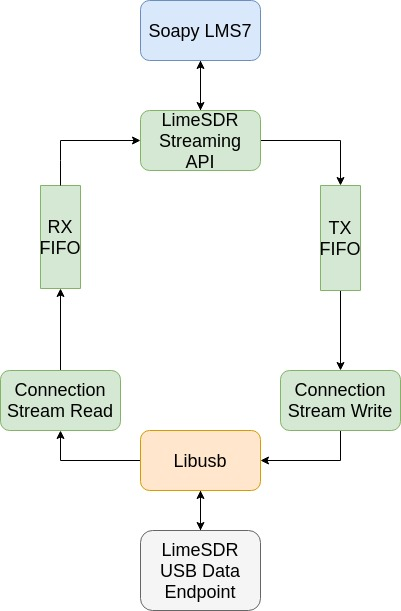
\includegraphics[scale=0.6]{Software_Architecture.jpg}
\caption{LimeSDR USB software architecture}
\end{figure}

\begin{itemize}
\item{\textit{TX Data Path:} Stream data from GNURadio is passed through Soapy drivers to the LimeSDR Streaming API. The API unwraps the data and the control flags and pushes it to the TX-FIFO. It also does the necessary data representation translation depending on the data format of the streamed data. For example, in case of complex data, it changes 32 bit I and Q value representation of GNU Radio to 16 bit I and Q values representation.  The values are pushed to the respective TX stream channel buffers(TXFIFO). The connection stream initializes the TX buffers and fills them with data from the TXFIFO. The Write function structures the data into FPGA data packet structure((Figure \ref{fpga_packet})) and combines multiple such packets into predefined batch size(initially 4). The buffer is processed by libusb to create bulk transfer packet and finally streamed to output data endpoint.}

\item{\textit{RX Data Path: } The USB data is continuously streamed from the LimeSDR to the Connection stream buffers through libusb. The Read function waits for data to be available from a usb context for the endpoint it is listening to, then it transfer data from the endpoint, parses the FPGA packets (Figure \ref{fpga_packet}) to collect the data and pushes them to the RXFIFO. If the rx stream is configured to have particular receive time, it checks if that condition is satisfied. The LimeSDR streaming API collects the data from the RXFIFO and does the necessary data interpretation translation (reverse translation to the TX Data Path), finally streams the data to GNURadio. }
\end{itemize}

\subsection{LimeSDR USB packets and endpoints}
LimeSDR uses four different endpoints for USB data transfer, these endpoints as Data Endpoint and Control Endpoint for both input and output directions. The control endpoints are used for configuring and retrieving data from the LMS7002M and NIOS Core on the FPGA. Data packets are used for the streaming data. 
\begin{table}[h!]
\centering
\begin{tabular}{|c|c|}
\hline
Endpoint No. & Function\\
\hline
0x01 & Stream Data Output\\
0x81 & Stream Data Input\\
0x0F & Control Data Output\\
0x8F & Control Data Input\\
\hline
\end{tabular}
\caption{LimeSDR USB transfer endpoints}
\end{table}
It uses two different packet structures for the LMS7002M Control Packets and the Stream Data Packets. Depending on the control command, different number of bytes are packed into one data element and the maximum number of blocks in a single packet is defined. One LMS64C protocol packet (Figure \ref{lms_packet}) is maximum 64 bytes, if the data to be sent is larger than that then the data field is segmented into several packets. The block count gives the number of data element in a single packet. The FPGA contains 4080 bytes of data along with 8 bytes of counter data that can be used for timestamp on the TX packets. The Lime driver uses synchronous bulk transfer for LMS Control packets and asynchronous bulk transfers for the FPGA packets.
\begin{figure}[h!]
\centering
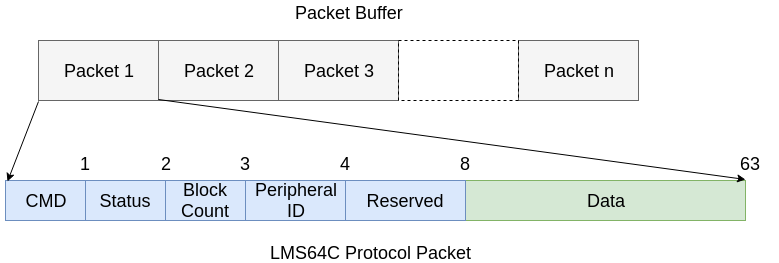
\includegraphics[width=\textwidth]{LMS64C_Packet.png}
\caption{LMS Control Packet Structure}
\label{lms_packet}
\end{figure}

\begin{figure}[h!]
\centering
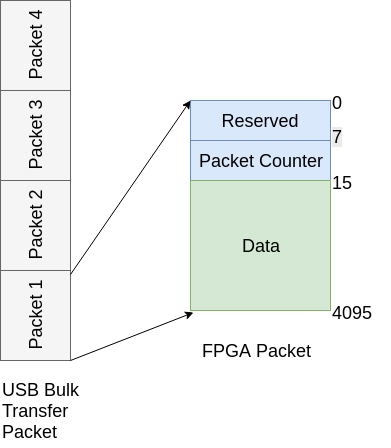
\includegraphics[scale=0.6]{FPGA_Packet.png}
\caption{FPGA Packet Structure}
\label{fpga_packet}
\end{figure}

\chapter{Methods}
This chapter introduces the quantitative methods used in the measurement of the timing delays. 
\section{Timing Analysis}
\begin{figure}[h!]
\centering
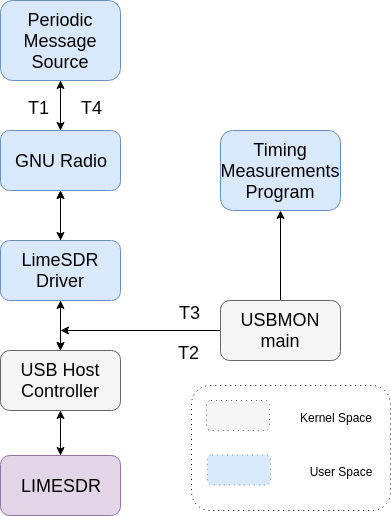
\includegraphics[scale=0.6]{Setup.png}
\caption{Overview of measurement setup}
\label{setup_overview}
\end{figure}
The project uses the Wime Project implementation of 802.15.4 MAC and PHY layers in GNU Radio. For the purpose of measurement of round trip latency, a loop back experimentation setup(Figure \ref{setup_overview}) was implemented. A periodic message source generates messages and notes down the time T1. It is then processed and modulated by the 802.15.4 MAC and PHY respectively and sent through the OSMOCOM transreceiver to the LimeSDR. The RX and TX ports of the LMS7002M has been shorted and hence the original sent message loopbacks through the FPGA and comes back to the GNU Radio and is demodulated and processed by the PHY and MAC blocks respectively and is ultimately received by the periodic message source and the time is noted as T4.

The usbmon kernel utility continuously monitors bus activity between the LimeSDR USB driver and USB Host Controller. It timestamps the transfers and generates event queues to be accessed from the user space. The timing measurements program parses the event queue to find the relevant packets and notes down their usbmon timestamps as T3 and T4 for transmit and receive packets respectively.  
\subsection{Message Source} \label{message_source}
A periodic message source block was implemented in the GNU Radio, it takes in the message length and time period as parameters. Figure \ref{message_source} shows the working of the message source with respect to time. The data length controls the duty cycle of the signal by varying $\Delta T_{tx}$, which is the time is requires to transmit the message through USB.\\

Everytime a message is sent and it receives a loopback, the block notes down the global time as T1 for transmit and T4 for receive respectively. Since the time noted should be compared with those from usbmon, \textit{gettimeofday} was selected as the preferred method. The time period was set such that the transmitted message is received before sending the next message.\\

\begin{figure}[h!]
\centering
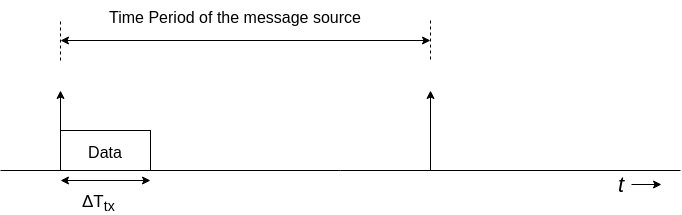
\includegraphics[width=\textwidth]{Message_Source.png}
\caption{Periodic Message Source}
\label{message_source}
\end{figure}
\subsection{Timing Measurements Program}
The timing measurements program uses ioctl to access the /dev/usbmonX character device. This allows the program to access the usbmon kernel utility event queue. The events are filtered to find packets with \textbf{0x01} \& \textbf{0x81} device endpoints. The data streams are parsed to find the relevant data fields from FPGA packets(Figure \ref{fpga_packet}), following that the data is converted from integer representation to complex floating point representation. The modulus of In Phase Sample's amplitude is used to determine if the data contained in the packet is useful or not. 

\begin{table}
\centering
\begin{tabular}{|c|c|}
\hline
USB Transfer Direction & Threshold Value  \\
\hline
|I| TX & 0.8\\
|I| RX & 0.2\\
\hline
\end{tabular}
\caption{Transfer Direction and Threshold Value}
\label{thres_table}
\end{table}

Analyzing the samples in the data stream, the samples threshold for actual data packets to as shown in Table \ref{thres_table}.  Once the packets have been analyzed, the sequence of events was studied to generate a state machine representation for the timing functionality.\\ 
The sequence follows the structure shown in figure \ref{sequence} if the condition mentioned about the time period in \ref{message_source} is satisfied. Since we want to measure the round trip delay, the time instant of the first TX and last RX packet as noted by T2 and T3 respectively needs to be measured. The difference between them gives the Kernel round-trip delay as measured by usbmon.    
\begin{figure}[h!]
\centering
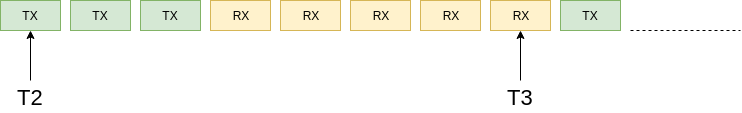
\includegraphics[width=\textwidth]{Sequence.png}
\caption{Sequence of valid data packet with time}
\label{sequence}
\end{figure}
\begin{figure}[h!]
\centering
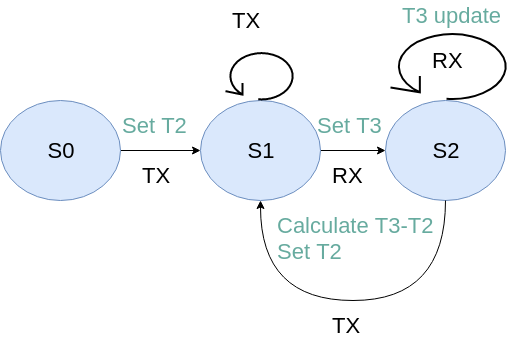
\includegraphics[scale=0.5]{State_Machine.png}
\caption{State Machine}
\label{state_machine}
\end{figure}

State Machine shown in Figure \ref{state_machine} controls the timing measurement function. It starts with state S0 and when it receives a TX event it sets T2 and moves to S1, further TX events don't update the value of T2 as we want the first TX event time. The state machine moves from S1 to S2 on a RX event, it sets the value of T3, further RX events updates the value of T3 as we want the time instant of the last RX event. On receiving TX event when at S2, it moves to S1, calculates $T3-T2$ and sets the value of T2.
\subsection{Results Correlation Method}
All the time instants are stored in Unix Time Format, a python script stores the values in separate arrays t1, t2, t3, t4 for GNU Radio Transmit Time, Kernel Transmit Time, Kernel Receive Time and GNU Radio Receive Time respectively. 

\begin{algorithm}[!h]
\caption{Time Data Correlation}
\begin{algorithmic}
\State {$T \gets $ Time Period of Message Source }
\State {$l \gets $ min(length of time arrays)}
\State $i \gets 0$
\For {$i < l $}
\If{($ t1[i]> t2[i]$ or $ t3[i]> t4[i]$)} \\
\hspace{1.35cm} delete $t1[i],t4[i]$
\ElsIf{$(t2[i]-t1[i]) > T $}
delete t2[i]
\ElsIf{$(t4[i]-t3[i]) > T $}
delete t3[i] 
\Else{ $i \gets i+1$ \\ \hspace{1.35cm} $l \gets $ min(length of time arrays) }
\EndIf
\EndFor
\end{algorithmic}
\end{algorithm}

Once the arrays have been compared to remove corrupt data, the mean and standard deviation of the respective arrays are found.

\chapter{Results and Analysis}
\subsection{Analytical Method}
The 802.15.4 PHY layer expands 1 byte of message data to 128 bytes, so the maximum packet length of 127 bytes becomes produces sample data of size
$127*128=16256 bytes=15.875KB$\\. The FPGA packet format adds 16 bytes overhead for every 4080 bytes so the overhead for 16256 bytes would be 64bytes. So the overall transfer size would be 16320 bytes. This would require four FPGA packets so the actual size of the USB transfer would be 16384 bytes
Now for sampling rate of 1MHz $\equiv$ 1MSPS, the actual data transfer is 1.5 MBps since the LMS7002M has 12 bits ADC and DAC. 
\begin{table}[!h]
\centering
\begin{tabular}{|c|c|}
\hline
Sampling Rate & USB Transfer delay \\
\hline
5 MHz & 4369.07 $\mu$s\\
10 MHz & 2184.53 $\mu$s\\
15 MHz & 1456.35 $\mu$s\\
20 MHz & 1092.27 $\mu$s\\
\hline
\end{tabular}
\caption{Analytical USB Transfer Delay}
\label{back_env}
\end{table}

\subsection{Experimental Results}
\begin{figure}
\centering
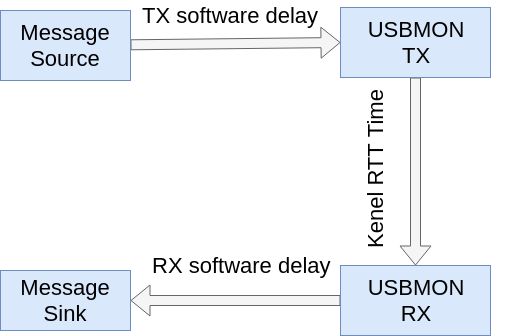
\includegraphics[scale=0.5]{results_setup.png}
\caption{Results Setup}
\label{res_set}
\end{figure}
Figure \ref{res_set} shows the different terminology used in the results, with the TX \& RX software delay is the delay caused by the GNU Radio and LimeSDR driver processing, the Kernel RTT Time includes the buffer delay in the LimeSDR and the USB communication delay. Total RTT Time = Kernel RTT Time + TX Software Delay + RX Software Delay. All the timing measurements are done on Lenovo Thinpad X240 with Dual-Core Intel® Core™ i5-4300U CPU @ 1.90GHz and 4GB RAM. The setup use Limesuite version 17.12.0 and gateware version 2.12.
\begin{table}
\centering
\label{res}
\begin{tabular}{|l|c|c|c|c|}
\hline
Sampling Rate(MHz)                                                  & 5    & 10   & 15   & 20   \\
\hline
Total RTT mean ($\mu$s)                                                      & 5360 & 3606 & 3065 & 4485 \\ \hline
Total RTT std deviation ($\mu$s)   & 326  & 472  & 262  & 1273 \\ \hline
Kernel RTT mean ($\mu$s)                                                     & 4113 & 1937 & 1354 & 762  \\ \hline
Kernel RTT std deviation ($\mu$s) & 1201 & 330  & 232  & 298  \\ \hline
TX chain mean ($\mu$s)                                                       & 470  & 675  & 831  & 1586 \\ \hline
TX chain std deviation ($\mu$s)    & 60   & 1165 & 186  & 860  \\ \hline
RX chain mean ($\mu$s)                                                       & 1100 & 1122 & 871  & 1769 \\ \hline
RX chain std deviation ($\mu$s)                                              & 472  & 1764 & 262  & 1036\\ \hline
\end{tabular}
\caption{Experimental results}
\end{table}



\subsection{Analysis}
\begin{itemize}
\item {The results show a monotonic drop in the kernel USB timings with increase in sampling rate and monotonic increase for RX and TX delay (Exception: 15 MHz). This indicates with increase in sampling rate, the buffers are getting overloaded and hence an increase in processing delay compared to bus communication delay.}
\item {Another thing that I noticed was at high sampling rate the round trip time increases with time, again pointing to buffer delay on the RX chain.}
\item {My measurement program becomes highly unstable at higher sampling rates, for example for 20MHz, I captured 610 packets of which I could correlate only 160 packets. This is mainly because the usbmon event queues overflow and hence my timing measurement program misses some relevant events and reports wrong timing information. One method I plan on using is flushing the buffers before the message source generates the message since each measurement is independent of the previous in a TDMA protocol.  }
\item {The analytical values for the RTT time( Table \ref{back_env}) is more than the actual value that usbmon reported(Table \ref{res}), my hypothesis is that this happens due to my assumption that all the data in the LimeSDR TX buffer is popped before the relevant RX data is popped back in the RX buffers on the LimeSDR side. But in actual operation even before all the TX data has been popped, the loopback data is being pushed to the RX buffers. This is demonstrated using figure \ref{staggering} where its shows the state of the RX and TX buffers with respect to time. \textit{t1} shows the instant when all the relevant data has been popped from the TX buffers and \textit{t2} shows the instant when the relevant RX data is popped from the buffers. For my assumption \textit{t1} should be equal to \textit{t2}, but here  $t2<t1$ hence the reported values are less than those of the analytical model. With increase in sampling rate the difference between t2 and t1 increases. There is a need to address this issue to ensure reliability of the measurement method.
\begin{figure}
\centering
\hspace{1cm}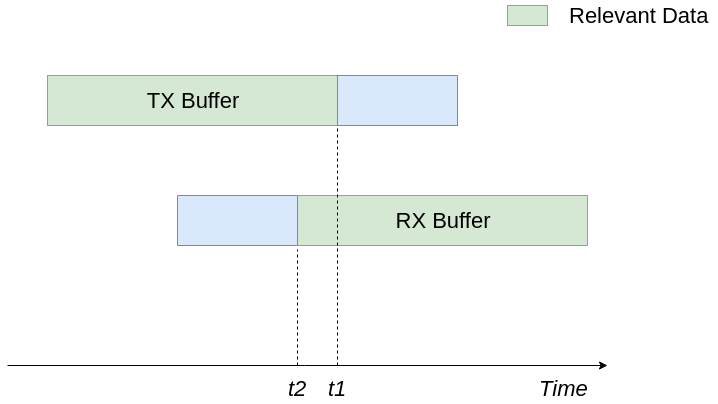
\includegraphics[scale=0.5]{Staggering.png}
\caption{Overlapping of buffers on LimeSDR}
\label{staggering}
\end{figure}
}
\end{itemize}

\chapter{What's next}

The project plan is presented in Gantt Chart format in figure \ref{plan}. According to my estimate I am one week behind the project plan.\\
\begin{itemize}
\item {Timing Analysis:\\
\begin{itemize}
\item {More data points to pinpoint the buffer delays.}
\item {Off-line processing of the USB data to pinpoint the time instant of maximum correlation between RX and TX data}
\item {Make individual measurements independent.}
\item {Solve the buffer overlap problem.}
\end{itemize}}
\item{Enabling deterministic timing: A key element for enabling TDMA protocols would be deterministic send and receive time of packets. So I would look at possible strategies.}
\item{Evaluation: Since I am looking at compression algorithms, it would be essential to find the compression ratio I am able to achieve with lossy and lossless compression. Also, I should concentrate on figuring out how these compression algorithms affect the performance of SDR systems. The strategies for deterministic timing needs to be evaluated for jitter to actual TDMA schedules.}
\end{itemize}
\begin{sidewaysfigure}
\centering
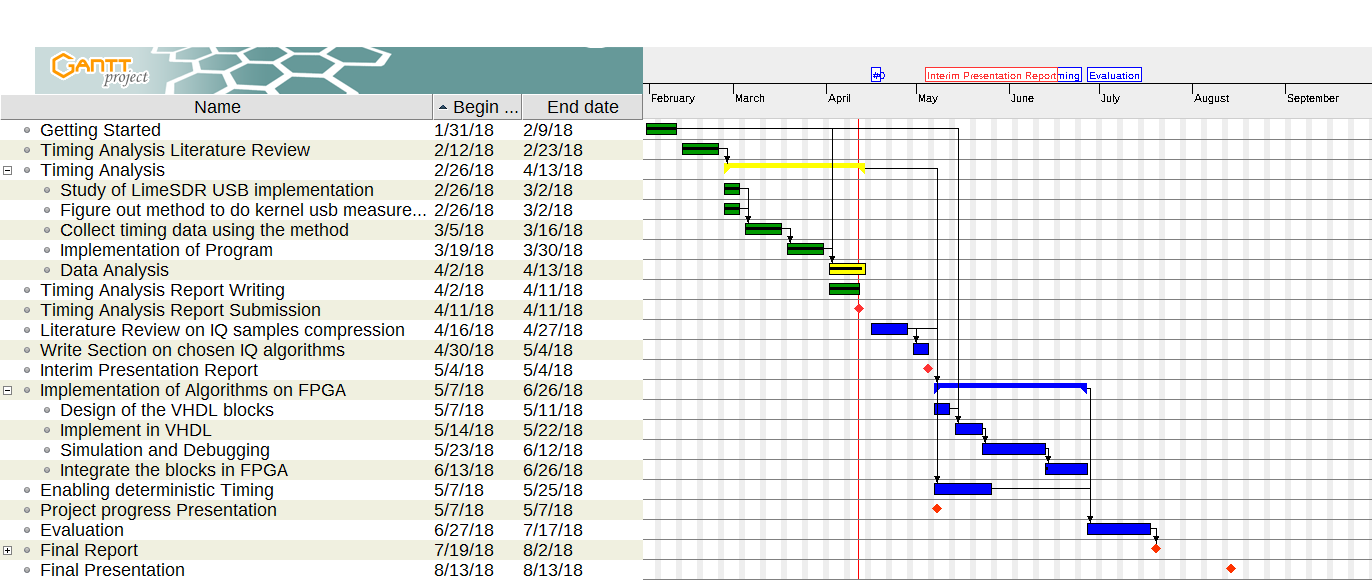
\includegraphics[width=\textheight]{Project_Plan.png}
\caption{Project Plan}
\label{plan}
\end{sidewaysfigure}

\printbibliography[heading=bibintoc] % Print the bibliography (and make it appear in the table of contents)

\appendix

% \chapter{Unnecessary Appended Material}

\end{document}
